\documentclass[../main.tex]{subfiles}
\begin{document}
\section{Results}\label{results}
%oppgave 5b)
\subsection{Euler and Verlet without oo}
In order to make sure that our algorithm is running correctly, we will start solving the differential equation using both Euler's and Verlet's method without using object oriented(oo) code. The algorithms used to calculate the two are located in the following folders (\href{https://github.com/kmaasrud/Project-5/tree/master/code/Earth-Sun_Euler-FWD}{(Euler)} and \href{https://github.com/kmaasrud/Project-5/tree/master/code/Earth-Sun_Verlet}{(Verlet)})

\begin{figure}[!h]
  \centering
  \makebox[\textwidth][c]{
  \begin{minipage}{0.6\textwidth}
        \centering
        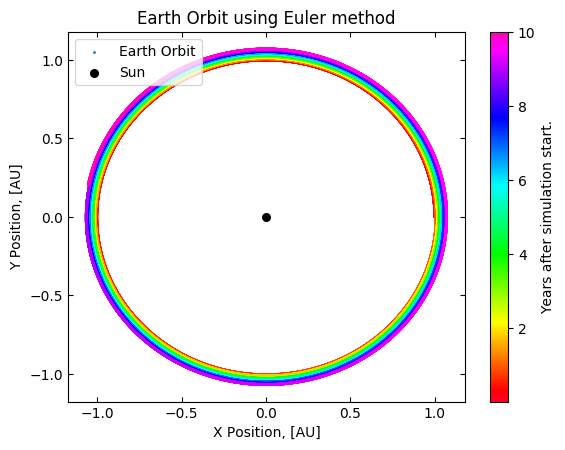
\includegraphics[width=1\textwidth]{EarthOrbit_Euler.png} % first figure itself
    \end{minipage}\hfill
    \begin{minipage}{0.6\textwidth}
        \centering
        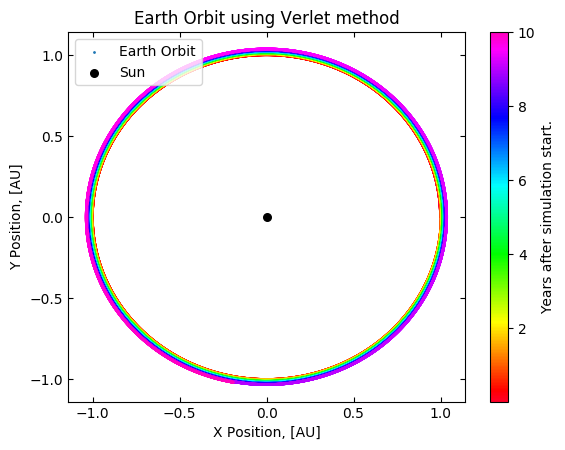
\includegraphics[width=1\textwidth]{EarthOrbit_Verlet.png} % second figure itself
    \end{minipage}
}
  \caption{Earth orbit around the Sun using Eulers method and Verlets method respectively }
  \label{fig:EarthOrbit_Euler_Verlet}
\end{figure}

%skriv litt om programflow

%oppgave 5c)


\subsection{Testing}
\subsubsection{Stability with varying timestep} \label{sec:results-test-timestep}
In the figures below we plotted Earths orbit over a thousand years with different timesteps.

\begin{figure}[!h]
  \centering
  \makebox[\textwidth][c]{
  \begin{minipage}{0.7\textwidth}
        \centering
        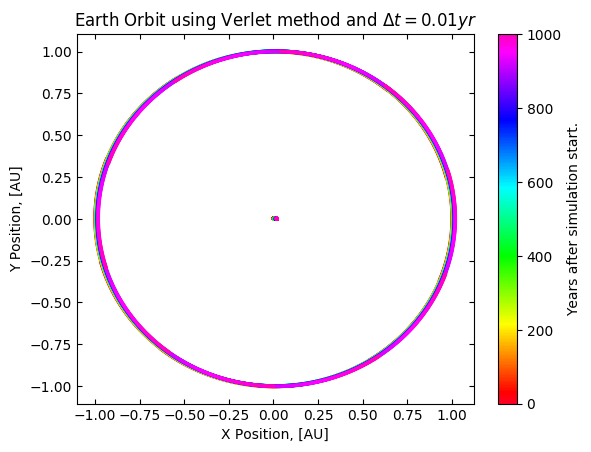
\includegraphics[width=1\textwidth]{/test/Earth-Sun_Test0-01.png} % first figure itself
    \end{minipage}\hfill
    \begin{minipage}{0.7\textwidth}
        \centering
        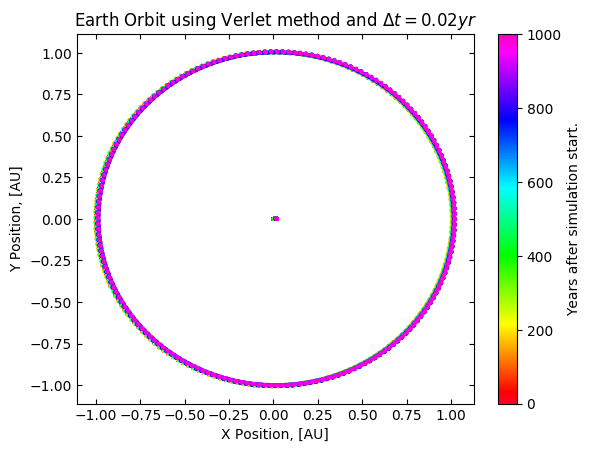
\includegraphics[width=1\textwidth]{/test/Earth-Sun_Test0-02.png} % second figure itself
    \end{minipage}
}
  \caption{Earth orbit with time steps $\Delta t = 0.01$years and $0.02$years respectively }
  \label{fig:results-Timestep1}
\end{figure}
\FloatBarrier
\begin{figure}[!h]
  \centering
  \makebox[\textwidth][c]{
  \begin{minipage}{0.7\textwidth}
        \centering
        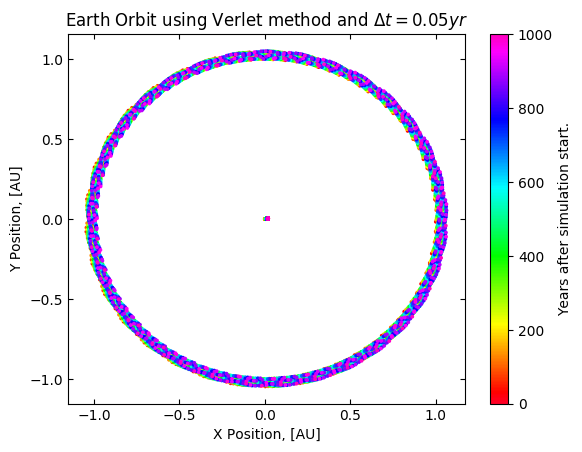
\includegraphics[width=1\textwidth]{/test/Earth-Sun_Test0-05.png} % first figure itself
    \end{minipage}\hfill
    \begin{minipage}{0.7\textwidth}
        \centering
        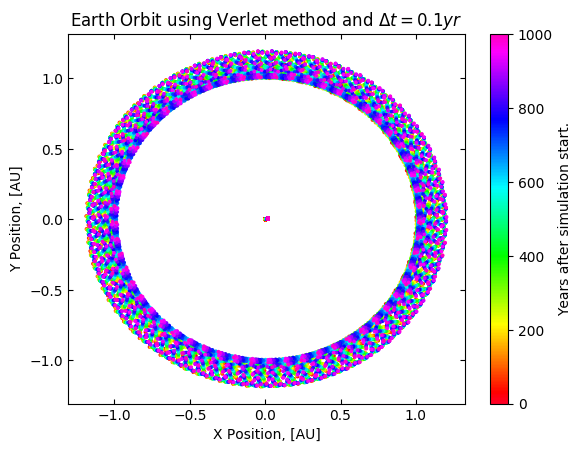
\includegraphics[width=1\textwidth]{/test/Earth-Sun_Test0-1.png} % second figure itself
    \end{minipage}
}
  \caption{Earth orbit with time steps $\Delta t = 0.05$year and $0.1$year respectively }
  \label{fig:results-Timestep2}
\end{figure}
\FloatBarrier

\subsubsection{Energy and angular momentum conservation}\label{sec:results-test-conservation}
In the figures below, kinetic energy and potential energy is plotted as a function of time in the system. We chose to simulate over a thousand years with a timestep of $\Delta t = 0.01$, as this gives the most stable results.
\begin{figure}[!h]
  \centering
  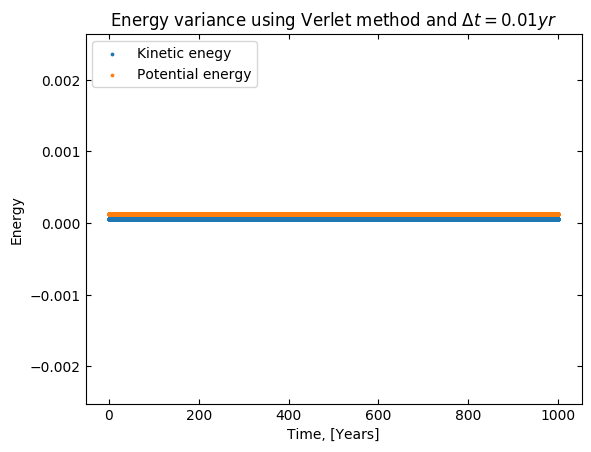
\includegraphics[width=1\textwidth]{/test/Energy_Test.png} % first figure itself
  \caption{Kinetic and Potential energy with timestep $\Delta t = 0.01$year.}
  \label{fig:results-Energies}
\end{figure}
\FloatBarrier

\subsubsection{Verlet vs. Euler}\label{sec:Verlet_VS_Euler}
\begin{table}[!h]
  \caption{Comparison of flops and time for the Verlet and Euler method for 100000 iterations over a period of 10 years}
  \centering
  \begin{tabular}{l r r}
                            &\textbf{Flops}&\textbf{Timing}\\
    Euler's method:          &10N&2580 ms\\
    Verlet's method:          &6N&2875 ms\\
  \end{tabular}
  \label{tab:EulervsVerlet}
  \end{table}
\FloatBarrier

%oppgave 5 d)
\subsection{Escape velocity}
By trail and error the escape velocity of planet Earth is somewhere between $2.8 \pi$ and $2.85 \pi$, which is pretty close to the theoretical value calculated below.
From section \ref{sec:theory} using equation \ref{eq:escapevelocity} to calculate the  theoretical value $$v_{esc-theoretical} = \sqrt{\frac{2\cdot4\pi^2\cdot1}{1}} = 2.83 \pi$$\

We also looked at what happens when changing the exponent of the denominator the force of gravity from 2 towards 3 with initial velocity $v_{initial,x} = 2.2\pi$. This is shown in the following plot.

\begin{figure}[h!]
  \centering
  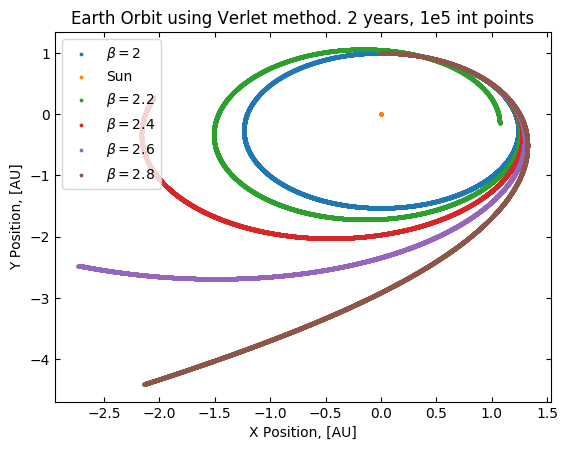
\includegraphics[width=0.8\textwidth]{Earth-Sun_beta.png}
  \caption{Escape velocity with increasing exponent of denominator of the gravitational force.}
  \label{fig:v_esc_beta}
\end{figure}

%oppgave 5e)
\subsection{Three-body problem- Sun, Earth and Jupiter.}
\begin{figure}[!h]
  \centering
  \makebox[\textwidth][c]{
  \begin{minipage}{0.7\textwidth}
        \centering
        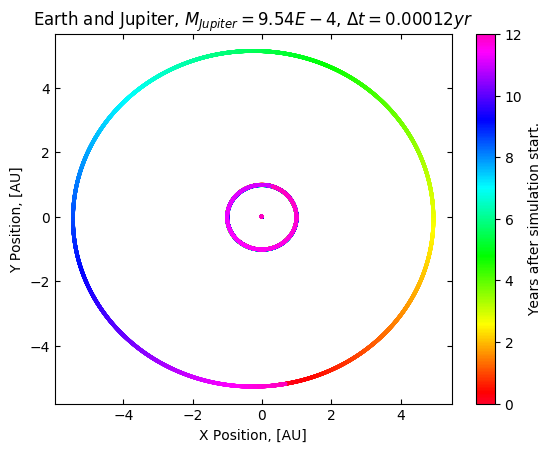
\includegraphics[width=1\textwidth]{jupiter-1.png} % first figure itself
    \end{minipage}\hfill
    \begin{minipage}{0.7\textwidth}
        \centering
        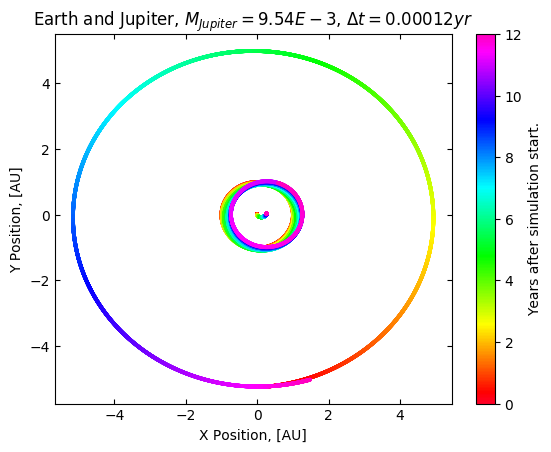
\includegraphics[width=1\textwidth]{jupiter-10.png} % second figure itself
    \end{minipage}}
  \caption{Positions of Sun in the middle, Earth second and outermost Jupiter calculated using the velocity Verlet method with with original mass of Jupiter and an increase of mass of a factor of 10 respectively}
  \label{fig:SunEarthJupiter10}
\end{figure}

\begin{figure}[!h]
  \centering
  \makebox[\textwidth][c]{
  \begin{minipage}{0.7\textwidth}
        \centering
        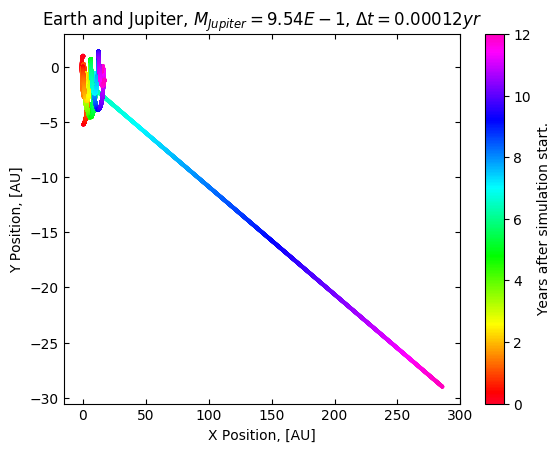
\includegraphics[width=1\textwidth]{jupiter-1000.png} % first figure itself
    \end{minipage}\hfill
    \begin{minipage}{0.7\textwidth}
        \centering
        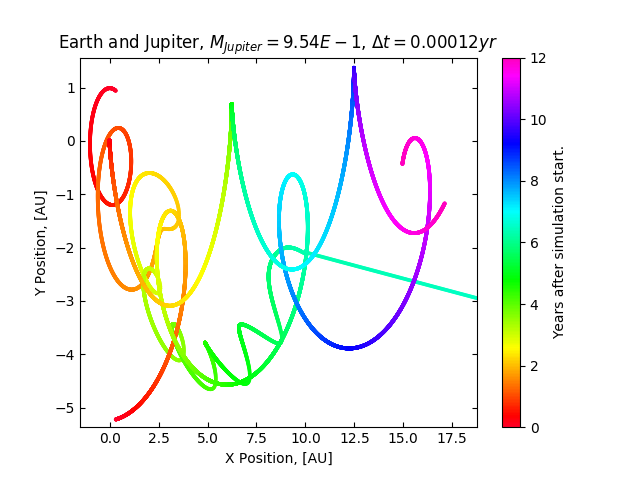
\includegraphics[width=1\textwidth]{jupiter-1000_Closeup.png} % second figure itself
    \end{minipage}}
  \caption{Positions of Earth and Jupiter using the velocity Verlet method with an increase of mass with a factor of 1000. The Sun starts at approximately (0,0)???, Jupiter starts at (0.0,-5)??? and Earth starts at (??????????). After som time, t$\approx 7$years Earth escapes the system. Picture to the right is a zoomed version of the first plot.}
  \label{fig:SunEarthJupiter10000}
\end{figure}

Stability Verlet solver with increased mass:



%oppgave 5f)
\subsection{The Solar system}
Finally we will add all the other planets to make the Solar system complete, still using the Verlet solver. Both the Earht, Jupiter and the Sun are in motion. Rather than having the origin in the postion of the sun, we set the center-off-mass of the three-body system in the origin. The inital velocity of the Sun is set to ?? in order to have the total momentum of the system to exactly zero.

\begin{figure}[!h]
  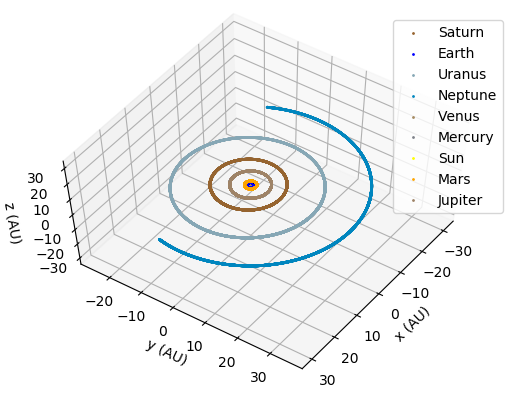
\includegraphics[width=0.7\textwidth]{allPlanets.png}
  \caption{All planets in The Solar System. Due to the large orbits of the outer planets, it is hard to plot the orbit of the inner planets, the Sun, Venus and Mercury without loosing information from the outermost planets.}
  \label{fig:allPlanets}
\end{figure}


Sammenlign resultetene med de tidligere.


\end{document}
